
\documentclass[11pt]{article}
\usepackage[table]{xcolor}
\usepackage[]{geometry} 
\usepackage{amsmath}
\usepackage{graphicx}

\usepackage{setspace}
\doublespacing

\usepackage{amssymb}
\usepackage{epstopdf}
\usepackage{inputenc}

\usepackage{dashrule}
\usepackage{float}
\usepackage{hyperref}
\usepackage{url}
\usepackage{mwe}
\usepackage{caption}

\usepackage[backend=biber,style=ieee]{biblatex}
\usepackage[toc]{appendix}
\usepackage[acronym]{glossaries}

\addbibresource{D1.bib}

\hypersetup{ linktoc=all}
\graphicspath{ {./images/} }

\makenoidxglossaries

\newacronym{ai}{AI}{Artifical Intelligence}
\newacronym{dnn}{DNN}{Deep Neural Network}
\newacronym{cnn}{CNN}{Convolutional Neural Network}
\newacronym{rnn}{RNN}{Recurrent Neural Network}
\newacronym{lstm}{LSTM}{Long Term Short Term Memory Network}


\newacronym{ncs}{NCS}{Neural Compute Stick}
\newacronym{tpu}{TPU}{Tensor Processing Unit}
\newacronym{vpu}{VPU}{Video Processing Unit}
\newacronym{gpu}{GPU}{Graphics Processing Unit}
\newacronym{apu}{APU}{Associative Processing Unit}
\newacronym{fpga}{FPGA}{Field Programmable Gate Array}
\newacronym{asic}{ASIC}{Application Specific Integrated Circuit}




\begin{document}
\title{%
	\bf Computing at the edge\\ 
	\large Deliverable 1: Final year Dissertation \\
	Bsc Computer Science: Artificial Intelligence}

\author{
	Sam Fay-Hunt | \texttt{sf52@hw.ac.uk}\\
	Supervisor: Rob Stewart | \texttt{R.Stewart@hw.ac.uk}
}

\maketitle

\pagebreak

\textbf{DECLARATION}\\
I, Sam Fay-Hunt confirm that this work submitted for assessment is my own and is expressed in
my own words. Any uses made within it of the works of other authors in any form (e.g., ideas,
equations, figures, text, tables, programs) are properly acknowledged at any point of their
use. A list of the references employed is included.\\
Signed: ......................\\
Date: .........................

\pagebreak

\textbf{Abstract:} a short description of the project and the main work to be carried out – probably
between one and two hundred words
\pagebreak

\tableofcontents
\thispagestyle{empty}
\pagebreak


\setcounter{page}{1}

\section{Introduction}
\emph{\textbf{Summarising the context of the dissertation project, stating the aim and objectives of the project, identifying the problems to be solved to achieve the objectives, and sketching
the organisation of the dissertation.}}

Edge devices have never been cheaper *citation*, stuff about how IoT devices are ubiquitous

Mention how there is an increasing trend to perform computing at the Edge - real time applications + privacy\\
These devices are often equipped with some form of AI application: Photo enhancment ect.\\
Online vs offline learning\\
Edge-side inference

These models can have a huge number of parameters so inference can sometimes be impractical.
\autocite{chenDeepLearningMobile2020} - ``see Table 1"

Issues with limited resource computation \autocite{szeEfficientProcessingDeep2017}

outline the document: We start with ..., then we cover x, y, and z ...

This dissertation is an investigation into the effect of pruning on inference in terms of latency and accuracy using 
hardware without specific optimisations for processing the resulting sparse matrices from pruning. (Reasoning for statement...). 

\pagebreak
\subsection{Background}
\emph{Discussing related work found in the technical literature and its relevance to your
project.}

This Section will be split into 4 subsections:\\
Hardware Memory architectures Section~\ref{subsec:hardwareArch} - brief stuff about this section\\
Edge Computing Section~\ref{subsec:edgeComputing} - stuff about edge comp\\
Deep Learning Section~\ref{subsec:deepLearning} - stuff\\
Compression Types Section~\ref{subsec:compressionTypes} - ...\\


\subsubsection{Hardware memory architectures}\label{subsec:hardwareArch}
\emph{
- Discuss VPU/TPU/APU/GPU/FPGA/ASIC memory arcitecture and how it handles matrix sparsity\\
- Show ineffectivity of pruning on hardware without optimisations for sparse matrices\\
}
The explosion of Deep Neural Network applications in recent years has prompted the production of a wave of specialised hardware architectures to improve the efficiency and compute of these kinds of workloads. The mainstay of this form of processing has been until recently been dominated by GPUs.\\

\subsubsection{Computing at the edge}\label{subsec:edgeComputing}
\emph{Some background on edge computing - maybe a detailed definition\\
 - Challenges of resource bound deep learning\\
 - Online vs offline learning\\}

\subsubsection{Neural networks \& Deep learning}\label{subsec:deepLearning}
\emph{
Types of deep learning \& inference\\
Deep Neural Network (DNN)\\
 - Layer structure (Input, Hidden, output)
 - Weight parameters updated using back-propagation
 - Feed Forwards\\
 - Feedback Nerual Network\\
 - Self-organizing Neural Network\\
Convolutional Neural Network (CNN)\\
 - A class of DNN\\
 - CNN consist of: Convolutional Layers, Pooling layers \& fully connected layers.\\
 - Convolutional Layers contain sets of filters/kernels\\
Recurrent Neural Network (RNN)\\
}

Neural networks are a subfield within the category of \Acrfull{ai} computing. Neural networkss are composed of layers of neurons that pass signals derived from weights through the network, this model of computing was inspired by our understanding of the human brain, see Fig.~\ref{fig:neuronLabeled} for a simple example, the weights can be seen corresponding to the synapes and the output of the neruon is labeled as the axon. All neruons in a Neural network have wieghts corresponding to their inputs, these weights are are intended to mirror the behavour of our synapses value scaling effect by performing a weighted sum operation. The neuron then applies an  non-linear activation function to the result, without which a Neural network would just be a linear algebra operation~\autocite{szeEfficientProcessingDeep2017}.



There are many popular deep learning network architectures, this document will focus primarily on the \Acrfull{cnn} and \Acrfull{rnn} architectures


\begin{figure}
    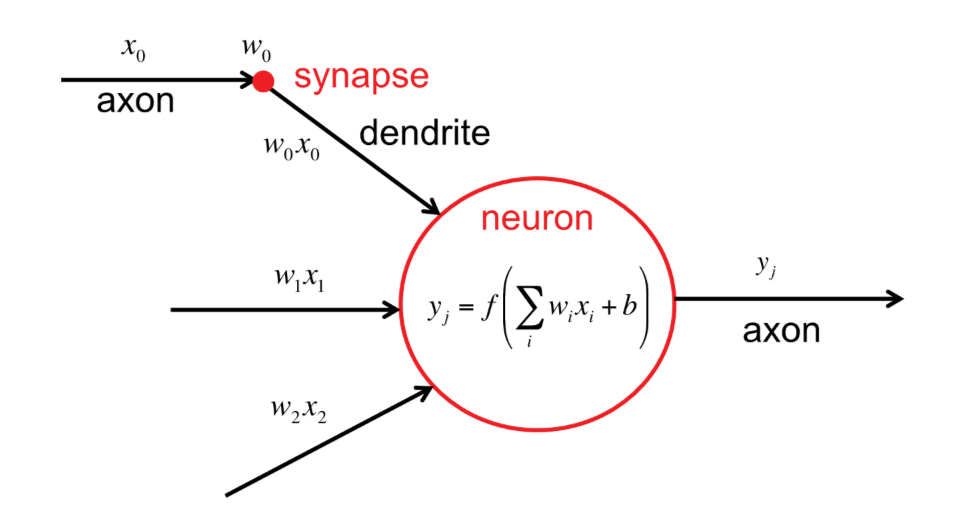
\includegraphics{Perceptron_efficient_proc.png}
    \caption{Neuron with corresponding biologically inspired labels.\\ \textbf{(Adopted figure from \autocite{szeEfficientProcessingDeep2017})}}
    \label{fig:neuronLabeled}
\end{figure}


\subsubsection{Compression types}\label{subsec:compressionTypes}
pruning\\
distillation\\
Quantization\\
Network design strategies\\
low-rank factorization\\

\pagebreak
\section{Research Methodology/ Requirements Analysis}
\subsection{Research Methodology}
This is required for research projects and should be linked
back to the project aim and objectives. It should describe the research methods that
will be employed in the project and the research questions that will be investigated.



Find baselines/benchmarks

How to perform pruneing

systematic benchmark framework

Look at underlaying storage mechanism of parameters in Network

perform some engineering of refactoring/altering these mechanisms


rerun systematic benchmarking framework





\subsection{Requirements Analysis}
This is required for technical projects and should be linked
back to the project aim and objectives. It should provide a detailed use case scenario
and suitable use

\pagebreak
\section{Design}
Initial software design/sketch of research Methodology

\pagebreak
\section{Evaluation Strategy}
Details of the evaluation and analysis to be conducted

\pagebreak
\section{Project Management}
\subsection{Timetable}

\subsection{Risk Analysis}

mention benchmarking NLP/NLG/Audio - text/text - audio models as a risk to the project

\subsection{Professional, Legal \& Ethical issues}

\pagebreak
\appendix
\section{Back matter}
\subsection{References}
\printbibliography

\subsection{Appendices}
to include additional material, consult with your supervisor.\\

\printnoidxglossary[type=acronym]
\printacronyms

\end{document}
